\section{Zmiany w architekturze projektu (AK)}
Przez zmiany w architekturze projektu autorzy rozumieją stopniowy rozwój zaimplementowanego przez nich w ramach pracy inżynierskiej rozwiązania. Rozwój ten obejmuje przede wszyskim uproszczenie powstałej hierarchii zależności między poszczególnymi elementami warstwy oprogramowania (rozumianymi zarówno jako repozytoria, jak i biblioteki), uczynienie systemu bardziej przystępnym dla użytkownika (np. poprzez nadanie komponentom nazw dobrze oddających ich przeznaczenie) oraz przygotowanie systemu pozwalającego w prosty sposób odtworzyć kod źródłowy w wersji bez wprowadzonych w ramach pracy magisterskiej modyfikacji (jako rodzaj zabezpieczenia przed skutkami potencjalnych błędów, które mogły zostać wprowadzone do oprogramowania podczas prac nad nim). Znaczna część zmian opisanych w niniejszej części pracy była możliwa do wprowadzenia z uwagi na trwające jednocześnie prace nad kodem źródłowym systemu GGSS i zmiany zachodzące w ich czasie.

\subsection{Wprowadzenie do problematyki}
Przeprowadzone przez autorów w ramach pracy inżynierskiej modyfikacje architektury systemu GGSS obejmowały przede wszystkim migrację projektu do systemu kontroli wersji Git, wprowadzenie spójnego nazewnictwa poszczególnych komponentów oraz zastosowanie funkcjonalności submodułów będącej częścią technologii Git do stworzenia hierarchicznej struktury repozytoriów (w odróżnieniu od pierwotnej, płaskiej architektury opartej o katalogi). Celem tych zmian było ułatwienie pracy nad pojedynczymi komponentami projektu oraz uczynienie struktury projektu przyjazną dla użytkownika, co zostało zdaniem autorów osiągnięte. 

Architektura stanowiąca punkt wyjściowy zmian wykonanych w ramach niniejszej pracy przedstawiona została na rysunku \ref{fig:old_structure} (z pominięciem repozytoriów pomocniczych, zawierających np. dokumentację). Zawarte na schemacie kolory obrazują rolę każdego modułu (zielony - repozytorium pomocnicze, czerwony - zależność zewnętrzna, żółty - aplikacja, fioletowy - sterownik urządzenia oraz niebieski - kod źródłowy oraz pliki nagłówkowe bibliotek). Projekt składał się zatem z 14 tworzących strukturę hierarchiczną repozytoriów, zawierających elementy takie jak: aplikacje, pomocnicze skrypty, infrastruktura budowania oraz kod źródłowy bibliotek implementujących poszczególne funkcjonalności systemu. W kontekście tej części pracy szczególnie istotne są repozytoria zawierające kod źródłowy bibliotek statycznych oraz pliki nagłówkowe, stanowiące trzon projektu (tzn. wykorzystywane przez aplikację \emph{ggss-runner}): \emph{ggss-lib}, \emph{ggss-software-libs}, \emph{ggss-hardware-libs}, \emph{ggss-util-libs} oraz \emph{ggss-misc} (repozytoria te oznaczone zostały na rys. \ref{fig:old_structure} kolorem niebieskim). Ich rola w pierwotnej wersji projektu prezentowała się następująco:
\begin{itemize}
    \item \textbf{\emph{ggss-hardware-libs}} - przechowywanie bibliotek odpowiedzialnych za obsługę urządzeń wchodzących w skład warstwy sprzętowej systemu GGSS. W pierwotnej wersji projektu były to następujące biblioteki statyczne:
    \begin{itemize}
        \item \emph{caenhv-lib} oraz \emph{caenn1470-lib} - odpowiedzialne za komunikację z zasilaczami wysokiego napięcia CAEN N1470
        \item \emph{mca-lib} oraz \emph{ortecmcb-lib} - odpowiedzialne za obsługę wielokanałowego analizatora amplitudy CAEN N957
        \item \emph{usbrm-lib} - odpowiedzialna za obsługę multipleksera sygnałów analogowych
    \end{itemize}
    \item \textbf{\emph{ggss-software-libs}} - przechowywanie bibliotek odpowiedzialnych za implementację wykorzystywanych przez system algorytmów i struktur danych związanych ściśle z warstwą oprogramowania (tzn. nie mających związku z warstwą sprzętową). W pierwotnej wersji projektu były to następujące biblioteki statyczne:
    \begin{itemize}
        \item \emph{xml-lib} - odpowiedzialna za implementację operacji odczytu oraz zapisu plików w formacie XML oraz operacji na strukturze drzewiastej powstałej w wyniku sparsowania zapisanych w tym formacie danych.
        \item \emph{fifo-lib} - odpowiedzialna za implementację prostej struktury danych, stanowiącej kolejkę typu FIFO (\emph{First In, First Out}) o ograniczonym rozmiarze.
        \item \emph{fit-lib} - odpowiedzialna za implementację operacji wykonywanych na zebranych przez system danych, w tym przede wszystkim za mechanizm dopasowania do nich krzywej.
        \item \emph{daemon-lib} - odpowiedzialna za implementację mechanizmu pozwalającego uruchomić aplikację \emph{ggss-runner} jako tzw. demon (ang. \emph{daemon}) - usługa działająca ,,w tle''
    \end{itemize}
    \item \textbf{\emph{ggss-util-libs}} - przechowywanie bibliotek, od których zależne są zarówno komponenty odpowiedzialne za obsługę warstwy sprzętowej projektu, jak i związane wyłącznie z warstwą oprogramowania. Innymi słowy, były to biblioteki wykorzystywane przez zawartość obu wyżej wymienionych repozytoriów, a zatem nie mogące znaleźć się w żadnym z nich. W pierwotnej wersji projektu były to następujące biblioteki statyczne:
    \begin{itemize}
        \item \emph{log-lib} - odpowiedzialna za implementację mechanizmu dziennika zdarzeń, zapisującego w plikach \lstinline{.log} informacje o zdarzeniach mających miejsce w systemie
        \item \emph{utils-lib} - odpowiedzialna za implementację pomniejszych funkcjonalności, takich jak konwersja między łańuchem znakowym a liczbą (przed pojawieniem się standardu C++11 tego typu funkcjonalności nie były częścią biblioteki standardowej)
        \item \emph{handle-lib} - odpowiedzialna za implementację wykorzystywanego w projekcie mechanizmu slotów i sygnałów
        \item \emph{thread-lib} - odpowiedzialna za implementację wykorzystywanego w projekcie mechanizmu wielowątkowości
    \end{itemize}
    \item \textbf{\emph{ggss-misc}} - przechowywanie plików nagłówkowych (niebędących cześcią żadnej z bibliotek statycznych) oraz plików \lstinline{.cmake} tworzących infrastrukturę budowania projektu
    \item \textbf{\emph{ggss-lib}} - przechowywanie kodu źródłowego zawierającego główną logikę systemu GGSS oraz przesyłane za pomocą protokołu DIM struktury danych
\end{itemize}

\begin{figure}[H]
\centering
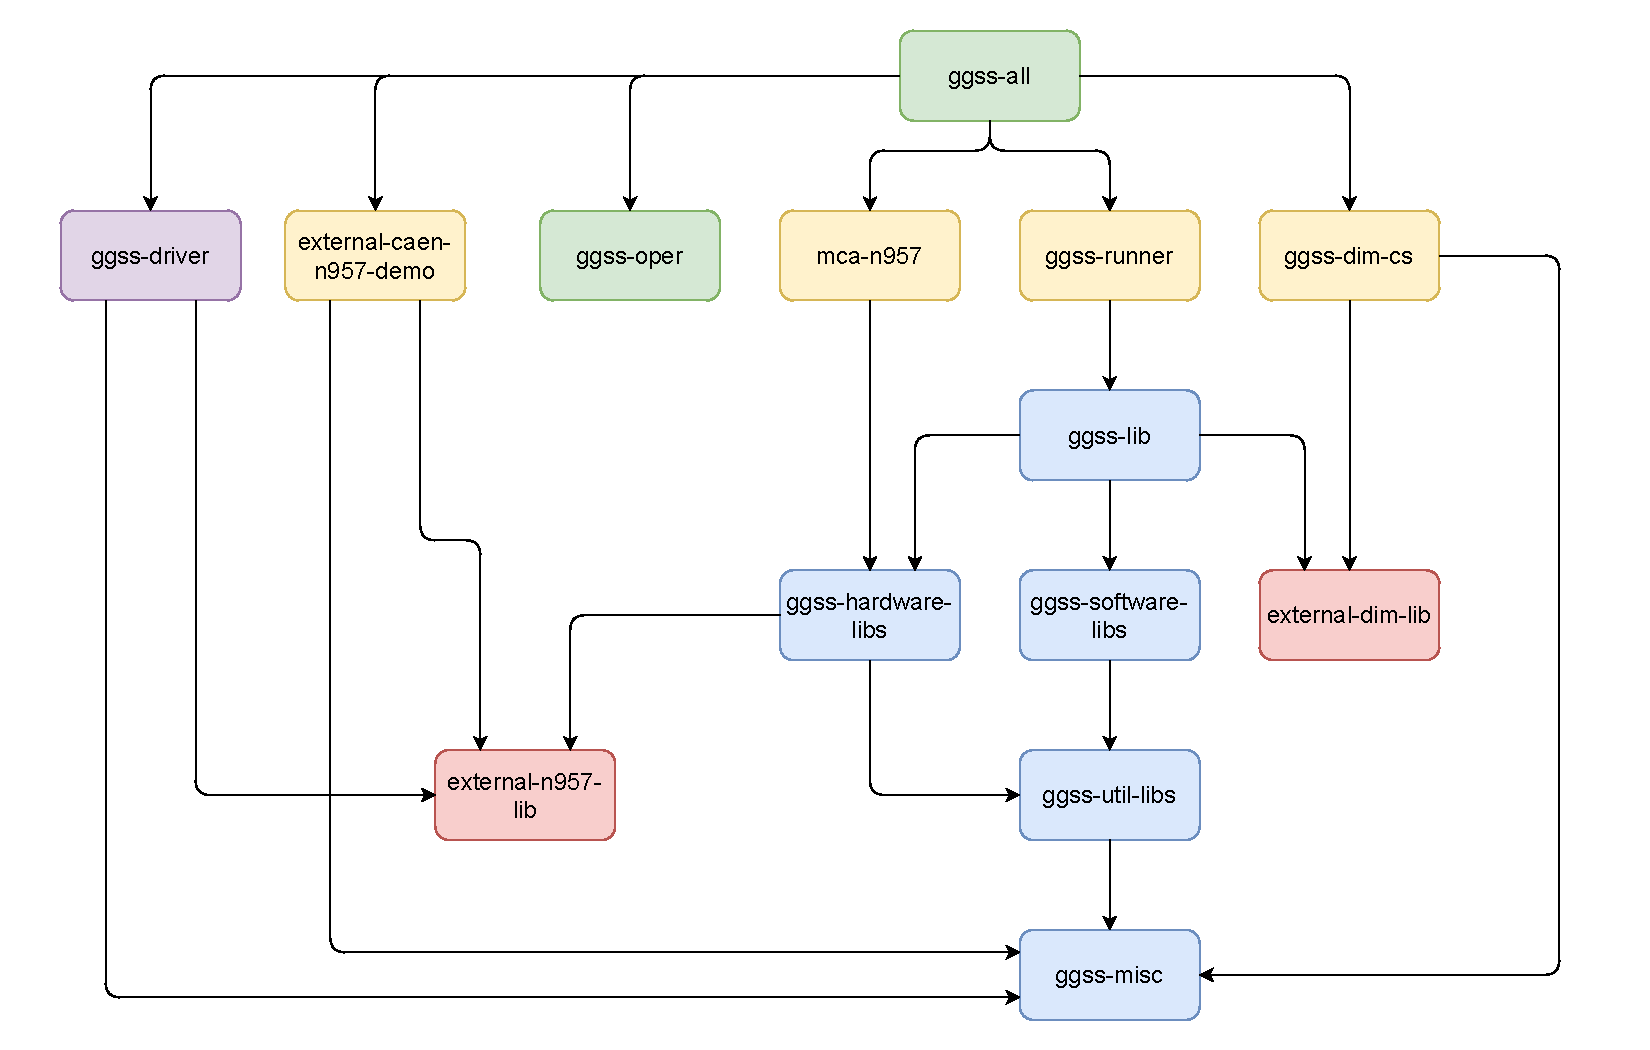
\includegraphics[width=\textwidth]{old_structure.pdf}
\caption{Architektura projektu przed wprowadzeniem modyfikacji (sytuacja wyjściowa). Groty strzałek wskazują repozytoria bazowe, kolory natomiast opisują rolę poszczególnych modułów: zielony oznacza repozytoria pomocnicze, żółty - aplikacje, czerwony - biblioteki zewnętrzne, fioletowy - sterownik a niebieski - biblioteki i pliki nagłówkowe projektu GGSS.}
\label{fig:old_structure}
\end{figure}

\subsection{Motywacja do wprowadzenia zmian}
Przygotowane przez autorów w ramach pracy inżynierskiej rozwiązanie było w pełni funkcjonalne, charakteryzowało się jednak pewnymi wadami i ograniczeniami, wynikającymi przede wszystkim z ograniczeń czasowych, niewielkiego doświadczenia autorów w pracy z projektem oraz istniejącego wtedy założenia o niemodyfikowaniu kodu źródłowego aplikacji i bibliotek wchodzących w skład projektu. Najważniejsze z występujących w tym rozwiązaniu problemów to:
\begin{itemize}
    \item głęboka hierarchia zależności, mająca negatywny wpływ na wydajność działania mechanizmu submodułów
    \item istnienie repozytorium \emph{ggss-misc}, zawierającego (poza szablonami CMake) elementy kodu źródłowego niepasujące do pozostałych bibliotek wchodzących w skład systemu: bazowe klasy wyjątków stosowanych w całym projekcie oraz flagi konfigurujące projekt w zależności od systemu operacyjnego (konieczność zastosowania tego typu zabiegu wynikła wprost z założenia o niemodyfikowaniu kodu źródłowego w czasie tworzenia pracy inżynierskiej)
    \item zachowanie oryginalnych nazw bibliotek i aplikacji, dostosowując je jedynie do przyjętej konwencji. Jedną z bibliotek wchodzących w skład projektu była biblioteka statyczna \emph{handle-lib}, odpowiedzialna za implementację mechanizmu slotów i sygnałów, na co, zdaniem autorów, jej nazwa nie wskazuje.
    \item wnioskowanie o zależnościach pomiędzy bibliotekami na podstawie dyrektyw preprocesora \emph{include} zawartych w kodzie źródłowym, a nie wykorzystywanych funkcjonalności, co wynikało z niewielkiego doświadczenia i wiedzy autorów na temat systemu podczas tworzenia pracy inżynierskiej oraz wspomnianego już założenia o niemodyfikowaniu kodu źródłowego.
    \item założenie o tworzeniu oddzielnego repozytorium dla każdej z występujących w projekcie aplikacji, niezależnie od jej rozmiarów, co ostatecznie znacznie skomplikowało powiązania pomiędzy repozytoriami (np. repozytoria \emph{external-caen-n957-demo} oraz \emph{mca-n957} charakteryzują się podobnymi zależnościami i oba zawierają niewielkie aplikacje, których zadaniem jest współpraca z wielokanałowym analizatorem amplitudy CAEN N957 - mogłoby być więc połączone w jedno repozytorium).
    \item brak łatwego sposobu na odtworzenie pierwotnej postaci kodu źródłowego - mechanizm ten nie był potrzebny na etapie pracy inżynierskiej, ponieważ nie dokonywano wtedy modyfikacji we wspomnianym kodzie.
\end{itemize}


\subsection{Uproszczenie architektury projektu}
Pierwszym podjętym przez autorów działaniem mającym na celu modyfikację struktury projektu była próba jej uproszczenia poprzez analizę zależności wewnętrzych systemu (tzn. zależności pomiędzy poszczególnymi bibliotekami). Prowadzone równolegle prace nad kodem źródłowym projektu pozwoliły autorom zaobserwować, iż pewna część występujących w nim dyrektyw preprocesora \lstinline{#include} nie oddaje w poprawny sposób faktycznej struktury zależności między bibliotekami. Najważniejszy przykład stanowi łańcuch zależności występujących pomiędzy biblioteką \emph{ggss-lib}, a bibliotekami \emph{caenhv-lib} oraz \emph{thread-lib}. W oryginalnej wersji projektu zależności między wymienionymi komponentami prezentowały się tak, jak na rysunku \ref{fig:dependency_problem_old}, tzn. bibliteka \emph{ggss-lib} zależna była od biblioteki \emph{caenhv-lib}, która natomiast zawierała dyrektywę \lstinline{#include} dołączającą plik nagłówkowy z biblioteki \emph{thread-lib}.


\savebox{\mybox}{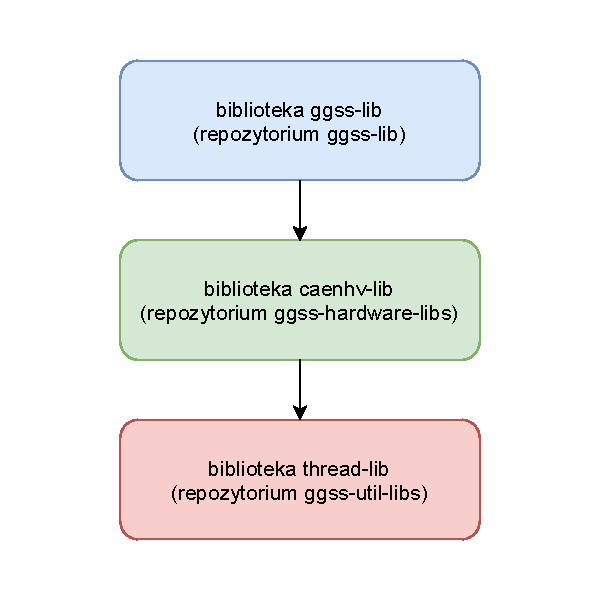
\includegraphics[width=0.40\textwidth]{dependency_problem_old.pdf}}

\begin{figure}[H]
\centering
\begin{subfigure}[t]{0.40\textwidth}
\centering
\usebox{\mybox}
\caption{Oryginalna struktura.}
\label{fig:dependency_problem_old}
\end{subfigure}
\hfill
\begin{subfigure}[t]{0.55\textwidth}
\centering
\vbox to \ht\mybox{%
    \vfill
    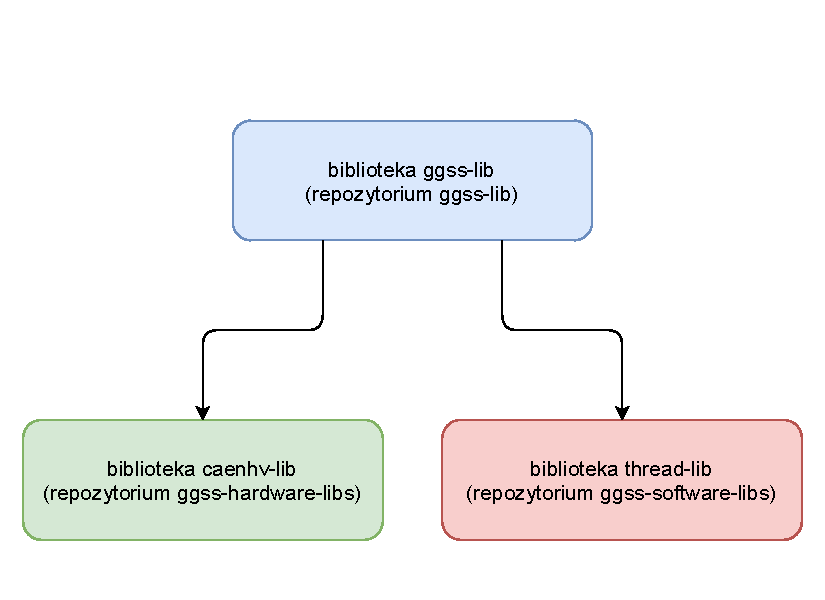
\includegraphics[width=\textwidth]{dependency_problem_solution.pdf}
    \vfill
}
\caption{Struktura po wprowadzeniu zmian.}
\label{fig:dependency_problem_solved}
\end{subfigure}

\caption{Zestawienie oryginalnej oraz nowej struktury zależności pomiędzy bibliotekami \emph{ggss-lib}, \emph{caenhv-lib} oraz \emph{thread-lib}. Groty strzałek wskazują w stronę modułów bazowych.}
\end{figure}

W rzeczywistości biblioteka \emph{caenhv-lib} nie wykorzystywała zawartości wspomnianego pliku nagłówkowego - pełniła jedynie formę swego rodzaju pośrednika, udostępniając znajdujące się tam klasy bibliotece \emph{ggss-lib}. Przeniesienie dyrektywy \lstinline{#include} do biblioteki \emph{ggss-lib} spowodowało, iż żadna z bibliotek wchodzących w skład repozytorium \emph{ggss-hardware-libs} nie zawierała zależności do biblioteki \emph{thread-lib}. Rozwiązanie to pozwoliło dokonać migracji tejże biblioteki, wraz z wykorzystywaną przez nią biblioteką \emph{handle-lib}, do repozytorium \emph{ggss-software-libs}, redukując tym samym liczbę bibliotek znajdujących się w repozytorium \emph{ggss-util-libs}. Rysunek \ref{fig:dependency_problem_solved} przedstawia w sposób schematyczny strukturę otrzymanego rozwiązania.

W związku z opisanymi powyżej zmianami ilość kodu źródłowego znajdującego się w repozytorium \emph{ggss-util-libs} znacznie spadła - pozostałe tam biblioteki \emph{log-lib} oraz \emph{utils-lib} charakteryzowały się niewielkim rozmiarem. Spowodowało to, iż jednoczesne istnienie modułów \emph{ggss-misc} oraz \emph{ggss-util-libs} (po wprowadzonych zmianach spełniających tą samą rolę przechowywania niewielkiej liczby komponentów wykorzystywanych przez wiele modułów projektu GGSS) przestało być uzasadnione. Kolejny etap wykonanych prac stanowiło więc przeprowadzenie integracji tychże repozytoriów - w tym celu zdecydowano się na likwidację modułu \emph{ggss-misc} po wcześniejszym przeniesieniu jego zawartości do \emph{ggss-util-libs}.

Migracja znajdujących się w repozytorium \emph{ggss-misc} plików \lstinline{.cmake} (modułów wykorzystywanych przez infrastrukturę budowania projektu) wymagała, poza wykonaniem trywialnej czynności przeniesienia katalogu, aktualizacji (na poziomie całego projektu) ścieżek wskazujących lokalizację tychże plików. Działanie to było konieczne, ponieważ narzędzie CMake wymaga od programisty, by wyspecyfikował on lokalizację modułów \lstinline{.cmake} dołączanych do projektu (np. za pomocą komendy \lstinline{include()}) poprzez dodanie ścieżki z ich lokalizacją do listy \lstinline{CMAKE_MODULE_PATH} (przykład wykorzystania tejże listy przedstawiony został na listingu \ref{lst:module_path}). Oznaczało to więc konieczność wykonania, w każdym module wykorzystującym pliki \lstinline{.cmake}, zmiany wspomnianej ścieżki tak, by wskazywała na katalog \emph{cmake-templates} w repozytorium \emph{ggss-util-libs}.

\begin{lstlisting}[
    language=cmake,
    caption={Przykładowy fragment pliku \lstinline{CMakeLists.txt}, obrazujący sposób użycia listy \lstinline{CMAKE_MODULE_PATH} w celu wskazania lokalizacji plików zawierających często wykorzystywane w projekcie, pomocnicze funkcje.},
    label={lst:module_path}
]
# Przypisanie pojedynczej wartości (zawierającej ścieżkę do katalogu
# cmake-templates, w którym znajdują się wykorzystywane w projekcie
# pliki .cmake) do listy CMAKE_MODULE_PATH
set(CMAKE_MODULE_PATH "${CMAKE_CURRENT_LIST_DIR}/../ggss-util-libs/cmake-templates")

# Dołączenie znajdujących się w katalogu cmake-templates plików .cmake
include(BuildStaticLibrary)     # ggss_build_static_library
include(SetupTests)             # ggss_setup_tests

# Wykorzystanie znajdującej się w pliku .cmake funkcji
ggss_build_static_library(
    TARGET_NAME "fifo"
)
\end{lstlisting}


Poza wspomnianymi plikami \lstinline{.cmake} w repozytorium \emph{ggss-misc} znajdował się katalog \lstinline{include}, zawierający trzy pliki nagłówkowe z kodem napisanym w języku C++:
\begin{itemize}
    \item pliki \lstinline{ggssExceptions.h} oraz \lstinline{HardwareException.h} zawierające klasy bazowe wyjątków wykorzystywanych w całym projekcie GGSS
    \item plik \lstinline{CompatibilityFlags.h}, zawierający flagi konfigurujące projekt w zależności od platformy docelowej (Windows lub Linux)
\end{itemize}
Pliki te nie wchodziły oryginalnie w skład żadnej z bibliotek projektu GGSS, nie mogły zostać do nich również dodane przez autorów podczas przygotowywania pracy inżynierskiej, ponieważ wymagałoby to modyfikacji kodu źródłowego systemu. Podczas przeprowadzanej w ramach niniejszej pracy migracji tych plików do repozytorium \emph{ggss-util-libs} zdecydowano się na likwidację katalogu \lstinline{include} i rozdysponowanie jego zawartości do istniejących lub nowych bibliotek. Plik \lstinline{CompatibilityFlags.h} przeniesiony został więc do biblioteki \emph{utils-lib}, natomiast na potrzebę dwóch pozostałych nagłówków przygotowana została nowa biblioteka \emph{exceptions-lib}.

Finalna struktura repozytorium \emph{ggss-util-libs} przedstawiona została na listingu \ref{lst:util_final}. Poza wspomnianymi do tej pory zmianami nowość stanowi katalog \lstinline{doxygen-config}, zawierający prosty plik konfigurujący działanie narzędzia Doxygen służącego do generowania dokumentacji programów napisanych w języku C++. Rozszerzenie projektu o możliwość generowania dokumentacji zostanie jednak opisane szczegółowo w dalszej części pracy.

\begin{lstlisting}[
    caption={Zawartość repozytorium \emph{ggss-util-libs} po wprowadzeniu opisanych zmian. Widoczne są biblioteki wchodzące w skład repozytorium: \emph{exceptions-lib}, \emph{log-lib} oraz \emph{utils-lib}, katalog \emph{cmake-templates} zawierający szablony wykorzystywane przez system budowania, katalog \emph{doxygen-config} zawierający konfigurację narzędzia Doxygen, nadrzędny plik \emph{CMakeLists.txt} służący do budowania wszystkich bibliotek w repozytorium oraz plik \emph{README.md} zawierający opis repozytorium.},
    label={lst:util_final}
]
.
|-- CMakeLists.txt
|-- README.md
|-- cmake-templates
|-- doxygen-config
|-- exceptions-lib
|-- log-lib
`-- utils-lib
\end{lstlisting}

Aby zachować możliwość wglądu w historię zmian przeprowadzanych w repozytorium \emph{ggss-misc} zdecydowano, że jego likwidacja polegać będzie na przeprowadzeniu archiwizacji oraz usunięciu z pozostałych modułów odniesień do niego. Udostępniany przez portal GitLab mechanizm archiwizacji polega na oznaczeniu repozytorium jako niemodyfikowalne i przeniesieniu go do osobnej zakładki w widoku organizacji. Dzięki takiemu rozwiązaniu repozytorium wciąć dostępne jest do wglądu (a zatem istnieje możliwość zbudowania tych wersji systemu GGSS, które korzystały z niego jako z submodułu), niemożliwy jest natomiast jego dalszy rozwój.


Poza wspomnianymi do tej pory repozytoriami zmianami objęte zostały ponadto moduły przechowujące aplikacje służące do testowania i obsługi urządzeń elektronicznych wchodzących w skład warstwy sprzętowej systemu GGSS. Motywacją do wprowadzenia modyfikacji była konieczność rozbudowy projektu o kolejne tego typu aplikacje - tworzenie dla każdej z nich osobnego repozytorium znacząco komplikowałoby strukturę projektu. Zdecydowano zatem, iż repozytoria \emph{mca-n957} oraz \emph{external-caen-n957-demo} zostaną dołączone do nowo powstałego repozytorium \emph{ggss-hardware-service-apps}, grupującego niewielkie programy służące do operowania na urządzeniach.


Poza zmniejszeniem progu wejścia do projektu poprzez uczynienie jego struktury prostszą, opisane do tej pory zmiany korzystnie wpłynęły na działanie mechanizmu submodułów systemu Git, na którym oparty został proces zarządzania zależnościami między repozytoriami w projekcie. Redukcja liczby repozytoriów i powiązań między nimi oraz zmniejszenie głębokości drzewa zależności (poprzez likwidację repozytorium \emph{ggss-misc}) miało pozytywny wpływ na wydajność systemu zarządzającego architekturą projektu. 



\subsection{Dodanie możliwości odtworzenia pierwotnej wersji kodu źródłowego}
Wprowadzanie zmian w kodzie źródłowym aplikacji, której jedną z najważniejszych cech jest jej niezawodność, stanowi znaczące ryzyko. Tego typu aplikacją jest program \emph{ggss-runner}, stanowiący trzon projektu GGSS, a którego źródła podlegały modyfikacjom w ramach opisanych w niniejszym manuskrypcie prac. Naturalnym było więc stworzenie mechanizmu pozwalającego na stosunkowo łatwy powrót do oryginalnej wersji aplikacji, tzn. takiej niezawierającej opisanych w niniejszej pracy zmian w kodzie źródłowym.

Możliwość odtworzenia pierwotnej wersji kodu źródłowego osiągnięta została poprzez utworzenie, dla każdego repozytorium biorącego udział w procesie budowania aplikacji \emph{ggss-runner}, specjalnej gałęzi nazwanej \emph{legacy}. Gałęzie te zawierają oryginalną wersję kodu źródłowego napisanego w języku C++, natomiast pozostałe elementy (infrastruktura budowania oraz ciągłej integracji i dostarczania) znalazły się tam w swoich najnowszych wersjach, co gwarantuje ich spójność w całym projekcie (a co za tym idzie, mogą być używane w taki sam sposób, jak na gałęzi głównej).

Opisanymi zmianami objęte zostały następujące repozytoria: \emph{ggss-all}, \emph{ggss-runner}, \emph{ggss-lib}, \emph{ggss-software-libs}, \emph{ggss-hardware-libs}, \emph{external-dim-lib}, \emph{external-n957-lib} oraz \emph{ggss-util-libs}. W przypadku repozytorów o nazwach zawierających przedrostek \emph{external-} zmiany te polegały jedynie na utworzeniu nowej gałęzi - zawartość bibliotek zewnętrznych nie była przez autorów pracy modyfikowana.

Ostatecznie więc zbudowanie aplikacji \emph{ggss-runner} w jej pierwotnej wersji jest bardzo proste, z poziomu repozytorium \emph{ggss-all} sprowadza się do wykonania komend zamieszczonych na listingu \ref{lst:legacy}. Dodatkowo, pliki \emph{README.md} stanowiące dokumentację poszczególnych repozytorów zostały na gałęziach \emph{legacy} odpowiednio zmodyfikowane, by opisywać obowiązującą tam procedurę budowania projektu oraz zawartość poszczególnych modułów.

\begin{lstlisting}[
    caption={Komendy pozwalające na pobranie kodu źródłowego oraz zbudowanie aplikacji \emph{ggss-runner} w jej oryginalnej wersji. },
    label={lst:legacy}
]
git clone ssh://git@gitlab.cern.ch:7999/atlas-trt-dcs-ggss/ggss-all.git &&
mkdir ggss-all-build &&
cd ggss-all &&
git checkout legacy &&
git submodule update --init --recursive &&
git submodule foreach --recursive git checkout legacy &&
cd ../ggss-all-build &&
python ../ggss-all/build.py --staticboost --buildtype release
\end{lstlisting}

\subsection{Pomniejsze zmiany}
Poza do tej pory opisanymi, wykonanych zostało kilka pomniejszych modyfikacji mających na celu szeroko pojętą poprawę jakości struktury projektu. Poniżej krotko opisane zostały trzy wybrane przez autorów modyfikacje, charakteryzujące się różnym poziomem skomplikowania, ale operujące na poziomie pojedynczych repozytoriów. 

\subsubsection{Archiwizacja repozytorium \emph{ggss-oper}}
Jednym z repozytoriów wprowadzonych przez autorów w ramach wykonywania pracy inżynierskiej był moduł \emph{ggss-oper}, zawierający skrypty oraz pliki konfiguracyjne stanowiące znaczną część infrastruktury przeznaczonej do użytkowania wraz z oprogramowaniem GGSS na maszynie docelowej. Zawartość tego repozytorium, nie stanowiąca wkładu wniesionego przez autorów niniejszej pracy w system, obejmowała m.in.: 
\begin{itemize}
    \item pierwsze wersje skryptów służących do przeprowadzania testów urządzeń wchodzących w skład warstwy sprzętowej projektu (napisane z wykorzystaniem języka Python)
    \item skrypty zarządzające stanem środowiska docelowego (np. ustawiające wymagane zmienne środowiskowe)
    \item skrypty zarządzające oprogramowaniem systemu GGSS, np. \lstinline{ggss_monitor.sh} pozwalający na uruchamianie, zatrzymywanie oraz sprawdzanie stanu aplikacji \emph{ggss-runner}
\end{itemize}
Wraz z postępami prac nad projektem, część z wymienionej powyżej zawartości zastąpiona została przez autorów pracy rozwiązaniami alternatywnymi (np. skrypty służące do przeprowadzania operacji na urządzeniach zastąpione zostały aplikacjami napisanymi w języku C++), pozostałe przeniesione zostały natomiast do repozytorium \emph{ggss-all}. Ostatecznie moduł został więc zarchiwizowany.


\subsubsection{Utworzenie biblioteki \emph{asyncserial-lib}}
Podczas prac nad kodem źródłowym bibliotek statycznych wchodzących w skład repozytorium \emph{ggss-hardware-libs} zaobserwowano, że w katalogach bibliotek \emph{usbrm-lib} oraz \emph{caenn1470-lib} zamieszczony został, poza właściwym dla nich kodem źródłowym, zestaw plików zawierających implementację asynchronicznej komunikacji z urządzeniami za pomocą interfejsu szeregowego. Ponieważ znalezione w obu przypadkach pliki nie różniły się od siebie, i jednocześnie stanowiły niezbędny element wspomnianych komponentów systemu (zawierały kluczową dla działania projektu funkcjonalność), zdecydowano o utworzeniu nowej biblioteki zawierającej omawiane pliki. Biblioteka nazwana została, zgodnie ze swoim przeznaczeniem, \emph{asyncserial-lib} i weszła w skład repozytorium \emph{ggss-hardware-libs}.


\subsubsection{Zmiana nazwy biblioteki \emph{handle-lib}}
Jedną z bibliotek będących częścią systemu GGSS była biblioteka \emph{handle-lib}, odpowiedzialna za implementację mechanizmu slotów i sygnałów. Oryginalnie biblioteka ta znajdowała się w repozytorium \emph{ggss-util-libs}, jednak wraz z postępem prac przeniesiona została, wraz z biblioteką \emph{thread-lib}, do repozytorium \emph{ggss-software-libs}. Nazwa biblioteki nie pozwalała użytkowniki domyślić się, jakie jest jej zastosowanie - z tego powodu zdecydowano się wprowadzić nową nazwę: \emph{sigslot-lib} (od angielskiego \emph{signals and slots}).


\subsection{Podsumowanie}
W ramach przeprowadzonych prac wykonane zostały zmiany pozwalające na uproszczenie architektury projektu, czyniąc ją przyjaźniejszą dla użytkownika. Finalna struktura przedstawiona została na rysunku \ref{fig:new_architecture} (podobnie jak w przypadku hierarchii wyjściowej - z pominięciem repozytoriów pomocniczych, nie wchodzących bezpośrednio w jej skład) - aktualnie składa się ona z 11 repozytoriów.

\begin{figure}[H]
\centering
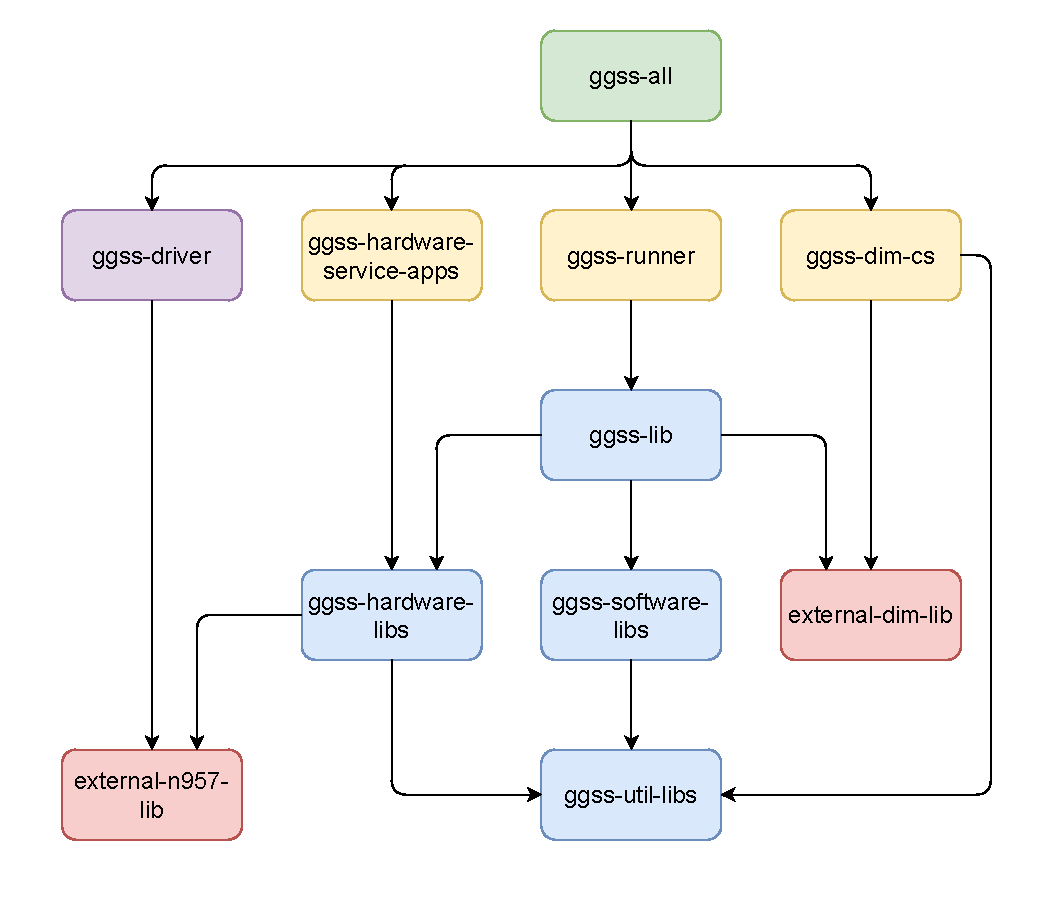
\includegraphics[width=\textwidth]{new_architecture.pdf}
\caption{Finalna struktura projektu, po wprowadzeniu wszystkich zmian opisanych w niniejszej pracy. Strzałki wskazują w stronę modułów bazowych. Widoczne jest znaczące uproszczenie struktury projektu względem wersji oryginalnej (rys. \ref{fig:old_structure}).}
\label{fig:new_architecture}
\end{figure}

Dla repozytoriów biorących udział w procesie budowania aplikacji \emph{ggss-runner} utworzone zostały ponadto gałęzie \emph{legacy}, zawierające kod źródłowy projektu bez wprowadzonych w ramach niniejszej pracy zmian - dzięki temu możliwy jest stosunkowo łatwy powrót do oryginalnej wersji aplikacji, co stanowi zabezpieczenie na wypadek wprowadzenia do jej źródeł błędów.